\subsection{Sensor noise measurement and estimation \label{sec:sensor_noise_measurement}}
In this section we will describe the measurement and estimation of the intrinsic noise of displacement sensors and inertial sensors, and how to model them.

\subsubsection{Displacement sensors \label{sec:displacement_sensors_baseline}}
Displacement sensors are usually relative displacement sensors that measure the differential displacement between the mounting point and an object.
Example sensors are Linear Variable Differential Transformer (LVDT) \cite{Akutsu:2021auw}, optical sensors and electromagnetic actuator (OSEM) \cite{Akutsu:2020efg, use_of_osems}, photo-reflective displacement sensors/photo sensors (PS), and optical levers (OpLev) \cite{sensing_matrices_oplev, length_sensing_oplev, optical_lever_for_kagra}.

In KAGRA's suspension, displacements sensors are non-contact sensors, i.e. the sensor doesn't affect the motion the sensing object, so the suspensions can swing freely to achieve passive seismic isolation.
However, this would mean that the sensing readout $Y$ contains the motion of the suspension, if the sensors are already installed, i.e.
\begin{equation}
	Y=X+N\,,
	\label{eqn:displacement_sensing_readout}
\end{equation}
where $X$ is the displacement readout and $N$ is the sensing noise.
Therefore, the only way to measure the sensor noise of the displacement sensors is to fix the suspension using the security structure, such that $X=0$.

Alternatively, we can measure the sensor noise before installation and apply proper calibration factors afterwards to convert the measurement units to displacement.
However, there might be error using this method, as there's no guarantee that the sensor noise retains the same before and after installation (or outside/inside vacuum/chamber).

Now, the aforementioned two methods can only be done before/during the installation stage.
If sensors are installed and in operation, there's no way to use these methods to measure the sensor noise of the displacement sensors\footnote{Can we use a three-channel correlation method?}.
But, approximation can still be done if have a model of the sensor noise.
This will be discuss in Sec.~\ref{sec:noise_modeling_baseline}.

\subsubsection{Inertial sensors \label{sec:inertial_sensors_baseline}}
In this section, we will describe techniques using correlation methods to measure sensor noise of inertial sensors \cite{technique_for_measurement_of_the_noise, Sleeman2006ThreeChannelCA}. Please also refer to appendix~\ref{appendix:spectral_density} for definitions and properties related to spectral densities.

Unlike displacement sensors, inertial sensors are self-contained sensors that are mounted to an object, whose motion are to be measured.
Some example sensors are geophone \cite{Sekiguchi:2016bmv}, accelerometers \cite{status_of_acc_development_2}, and seismometers \cite{trillium_compact_120-sv1}.
Calibrated inertial sensors output the velocity or the acceleration of the object which is relative to the object's inertial frame.
Because of this, sensor noise of inertial sensors cannot be measured by measuring the readouts when fixing suspension, as the readouts become the motion of the ground (effectively making the inertial sensor a seismometer.).
In any case, The readout of a single inertial sensor will be no different from that of Eqn.~\eqref{eqn:displacement_sensing_readout}.
Therefore, we cannot use single readout to estimate the sensor noise.

Instead, we rely on using multiple sensors and use correlation methods.
Now, let's assume that we have multiple sensors that reads $Y_i$, where $i=1,2,...K$, and $K$ is the total number of sensors.
If we place the sensors at the same location, they measure the same signal $X$.
Then, the sensor readouts becomes
\begin{equation}
	Y_i = XH_i + N_i\,,
	\label{eqn:inertial_sensing_readout}
\end{equation}
where $H_i$ is the transfer function from the signal to the sensing readout and $N_i$ is the sensor noise of the $i^\mathrm{th}$ sensor.

\paragraph{Two-channel method}

If we have sensors that have the same response and same power spectral density, then we can determine the sensor noises using only two sensors \cite{technique_for_measurement_of_the_noise}.
Let's say the sensors are well calibrated such that $H_i=1$, and assuming that the signal $X_i$ is uncorrelated with the noise $N_i$, then the power spectral density of the sensor readouts is simply
\begin{equation}
	P_{y_iy_i}(f) = P_{xx}(f) + P_{n_i n_i}(f)\,,
\end{equation}
and the cross power spectral density (CPSD) between $Y_i$ and $Y_j$ is
\begin{equation}
	\begin{split}
		P_{y_iy_j}(f) &= P_{xx}(f) + P_{xn_i}(f) + P_{n_ix}(f) + P_{n_in_j}(f) \\
		&= P_{xx}(f)\,,
	\end{split}
	%	\label{eqn:p_yi_yj}
\end{equation}
where we assume $X$, $N_i$, and $N_j$ are uncorrelated for $i\neq j$ so their CPSDs are identically zero.
Following that, the coherence between sensor readout $Y_i$ and $Y_j$ is
\begin{equation}
	\begin{split}
		C_{y_iy_j}(f) &= \frac{\left\lvert P_{y_iy_j(f)}\right\rvert^2}{P_{y_iy_i}(f)P_{y_jy_j}(f)}\\
		&= \frac{P_{xx}(f)^2}{\left[P_{xx}(f)+P_{n_i n_i}(f)\right]\left[P_{xx}(f)+P_{n_j n_j}(f)\right]} \,.
	\end{split}
	\label{eqn:coherence_yi_yj}
\end{equation}
Here, if the power spectral densities of $N_i$ and $N_j$ is the same, i.e. $P_{n_in_i}(f)=P_{n_jn_j}(f)$, Eqn.~\eqref{eqn:coherence_yi_yj} further simplifies to
\begin{equation}
	C_{y_iy_j}(f) = \frac{P_{xx}(f)^2}{\left[P_{xx}(f)+P_{n_i n_i}(f)\right]^2}\,.
\end{equation}
Substituting $P_{y_i y_i}(f) = P_{xx}(f) + P_{n_i n_i}(f)$ and rearranging, we get
\begin{equation}
	\begin{split}
		C_{y_iy_j}(f)^\frac{1}{2} &= \frac{P_{xx}(f)}{P_{y_iy_i}(f)} \\
		P_{y_iy_i}(f)C_{y_iy_j}(f)^\frac{1}{2} &= P_{xx}(f) \\
		P_{y_iy_i}(f)\left[1-C_{y_iy_j}(f)^\frac{1}{2}\right] &= P_{y_iy_i}(f) - P_{xx}(f)\,.
	\end{split}
\end{equation}
Substituting $P_{n_i n_i}(f) = P_{y_i y_i}(f) - P_{xx}(f)$, finally we obtain
\begin{equation}
	\boxed{
		P_{n_i n_i}(f) = P_{y_iy_i}(f)\left[1-C_{y_iy_j}(f)^\frac{1}{2}\right]
	}\,\ .
	\label{eqn:p_ni_ni_2channel}
\end{equation}
And again, note that Eqn.~\eqref{eqn:p_ni_ni_2channel} only works if the two sensors are identical, i.e. having the same noise spectral density and are inter-calibrated such that the read a same coherent signal.

\paragraph{Three-channel method}

Now, if we don't have identical sensors, which is generally true, then we have to rely on a three-channel method that uses 3 sensors \cite{Sleeman2006ThreeChannelCA}.
The advantage of this method is that we can estimate the sensor noise of each individual sensor, even if they have completely different calibration, dynamics, and noise spectrum.
Recall the sensor readout Eqn.~\eqref{eqn:inertial_sensing_readout}, the cross power spectral density between the $i^\mathrm{th}$ and $j^\mathrm{th}$ sensors is
\begin{equation}
	P_{y_iy_j}(f) = P_{xx}(f)H_iH_j^*\,,
\end{equation}
where $H_j^*$ denotes the complex conjugate of the transfer function $H_j$ and $i\neq j$.
Again, we have assumed that the coherent signal $X$, the noises $N_i$ and $N_j$ are uncorrelated such that their CPSDs are zero.
If we have three sensors then we can have two cross power spectral density, $P_{y_iy_k}(f)$ and $P_{y_jy_k}(f)$, and $i,j,k=1,2,3$ and $i\neq j\neq k$.
Then, taking the ratio gives
\begin{equation}
	\frac{P_{y_iy_k}(f)}{P_{y_jy_k}(f)} = \frac{H_i}{H_j}\,.
	\label{eqn:p_yi_yj}
\end{equation}
The ratio between the PSD $P_{y_iy_i}(f)$ and CPSD $P_{y_jy_i}$ reads
\begin{equation}
	\begin{split}
		\frac{P_{y_iy_i}(f)}{P_{y_jy_i}(f)} &= \frac{P_{xx}(f)H_iH_i^*\ + P_{n_in_i}(f)}{P_{xx}(f)H_jH_i^*} \\
		&= \frac{H_i}{H_j} + \frac{P_{n_in_i}(f)}{P_{y_jy_i}(f)}\,.
	\end{split}
	\label{eqn:p_yi_yi_on_p_yj_yi}
\end{equation}
Now, substituting Eqn.~\eqref{eqn:p_yi_yj} into Eqn.~\eqref{eqn:p_yi_yi_on_p_yj_yi} and rearranging gives
\begin{equation}
	\boxed{
		P_{n_in_i}(f) = P_{y_iy_i}(f) - \frac{P_{y_iy_k}(f)}{P_{y_jy_k}(f)}P_{y_jy_i}(f)\,
	}\,\ ,
	\label{eqn:p_ni_ni_3channel}
\end{equation}
which expresses the PSD of the noise as the PSDs and the CPSDs of the measurements.

\textbf{Warning. The following paragraph is not from \cite{Sleeman2006ThreeChannelCA}, but is seemingly important.}

\paragraph{Modified three-channel method}

Let's inspect Eqn.~\eqref{eqn:p_ni_ni_3channel}.
Eqn.~\eqref{eqn:p_ni_ni_3channel} is an equation as written in \cite{Sleeman2006ThreeChannelCA} but is seemingly not directly implementable.
The second term in Eqn.~\eqref{eqn:p_ni_ni_3channel} are products of cross power spectral densities.
If we look at Eqn.~\eqref{eqn:p_yi_yj}, the CPSDs are expressed in products of transfer functions, are complex-valued series.
These features should note exist in a power spectral density as it's expected to be a real-valued frequency series.
To fix this problem, we propose to modify Eqn.~\ref{eqn:p_ni_ni_3channel} by taking the absolute value of the second term, i.e.,
\begin{equation}
	\begin{split}
		P_{n_in_i}(f) &\approx P_{y_iy_i}(f) - \left\lvert\frac{P_{y_iy_k}(f)}{P_{y_jy_k}(f)}P_{y_jy_i}(f)\right\rvert\\
		&= P_{y_iy_i}(f) - \frac{\left\lvert P_{y_iy_k}(f)\right\rvert}{\left\lvert P_{y_jy_k}(f)\right\rvert}\left\lvert P_{y_jy_i}(f)\right\rvert\,.
	\end{split}
	\label{eqn:modified_three_channel_noise}
\end{equation}
Recall that the definition of coherence function, first line of Eqn.~\eqref{eqn:coherence_yi_yj}, we can write express the absolute value of a cross power spectral density as
\begin{equation}
	\left\lvert P_{y_iy_j}(f)\right\rvert = C_{y_iy_j}(f)^{\frac{1}{2}}P_{y_iy_i}(f)P_{y_jy_j}(f)\,
	\label{eqn:absolute_cpsd}
\end{equation}
where $C_{y_iy_j}(f)$ is the coherence function between readouts $Y_i$ and $Y_j$.
Substituting Eqn.~\eqref{eqn:absolute_cpsd} into Eqn.~\eqref{eqn:modified_three_channel_noise} gives
\begin{equation}
	\boxed{
		P_{n_in_i}(f) \approx 	P_{y_iy_i}(f)\left[1-\left(\frac{C_{y_iy_k}(f)}{C_{y_jy_k}(f)}C_{y_jy_i}(f)\right)^\frac{1}{2}\right]
	}\,\ ,
	\label{eqn:modified_p_ni_ni_3channel}
\end{equation}
which is an expression very similar to Eqn.~\ref{eqn:p_ni_ni_2channel} and has convenient properties, i.e. coherence functions are symmetric $C_{ij}(f) = C_{ji}(f)$.

\subsubsection{Examples}

We will demonstrate the use of these correlation methods in the form of a Jupyter notebook.
The notebook is available in the Kontrol library \cite{kontrol_noise_estimation}, where Eqn.~\eqref{eqn:p_ni_ni_2channel}, ~\eqref{eqn:modified_three_channel_noise}, and \eqref{eqn:modified_p_ni_ni_3channel} are coded.
We will copy important results from the \href{https://kontrol.readthedocs.io/en/latest/tutorials/noise_estimation_using_correlation_methods.html}{notebook}.

\begin{figure}[!h]
	\centering
	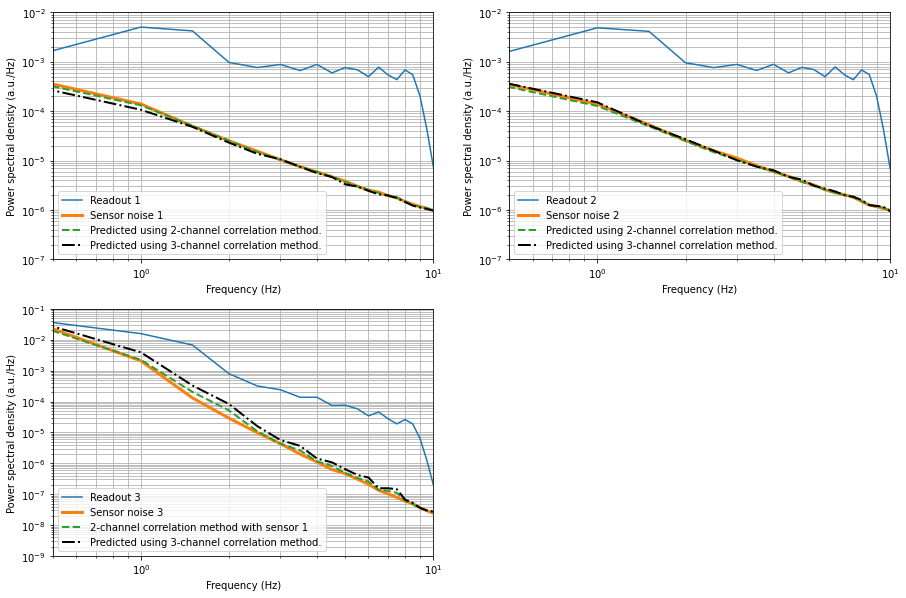
\includegraphics[width=1\linewidth]{figures/noise_estimation_using_correlation_methods}
	\caption{A comparison between the two-channel method and three-channel method.}
	\label{fig:noiseestimationusingcorrelationmethods}
\end{figure}
Fig.~\ref{fig:noiseestimationusingcorrelationmethods} shows a comparison between the two correlation methods from the notebook.
Sensor 1 and 2 has the same dynamics and noise PSDs, while sensor 3 has a completely different dynamics and noise PSD from the other two.
We used two-channel method to predict sensor noise 1 and 2, and used three-channel method for all of them.
We also used the two-channel method to predict sensor noise 3 using sensor 1 as a correlated sensor.
As shown in the figure, the predicted PSDs (shown in green dashed and dotted black lines) are very close to the actual sensor noises (shown in orange).
Here, we emphasize that using the two-channel method to predict self noise of sensor 3 is not a valid attempt as the other sensors don't have the same sensor dynamics and noise spectral density.
Hence, the green dashed line on the bottom left in Fig.~\ref{fig:noiseestimationusingcorrelationmethods} might be a fluke.
We used the same method to predict sensor noise 1 using sensor 3 as a correlated sensor and the prediction was clearly off (See the notebook for a figure).
